\section{TEST PROCEDURES}

In order to evaluate each of the discussed IPC methods, a test system was developed that incorporated a laptop, 100mbps wired network connection, a Raspberry Pi single board computer (SBC), and an OpenCM9.0 microcontroller board designed for command and control of dynamixel servomotors. The system transports messages over ethernet, serial, and USB. For consistency, the serial link was set to the same baud rate (9600) as the USB link. The objective of this test was to measure the round trip latency of a message by utilizing each of the aforementioned IPCs. Only one communication link (Link 1 or Link 2) varied for each test and UDP was selected as the control for the other. Figure \ref{fig:test block diag} below shows the overall system diagram of the test setup. 

\begin{figure}[thpb]
 \centering
 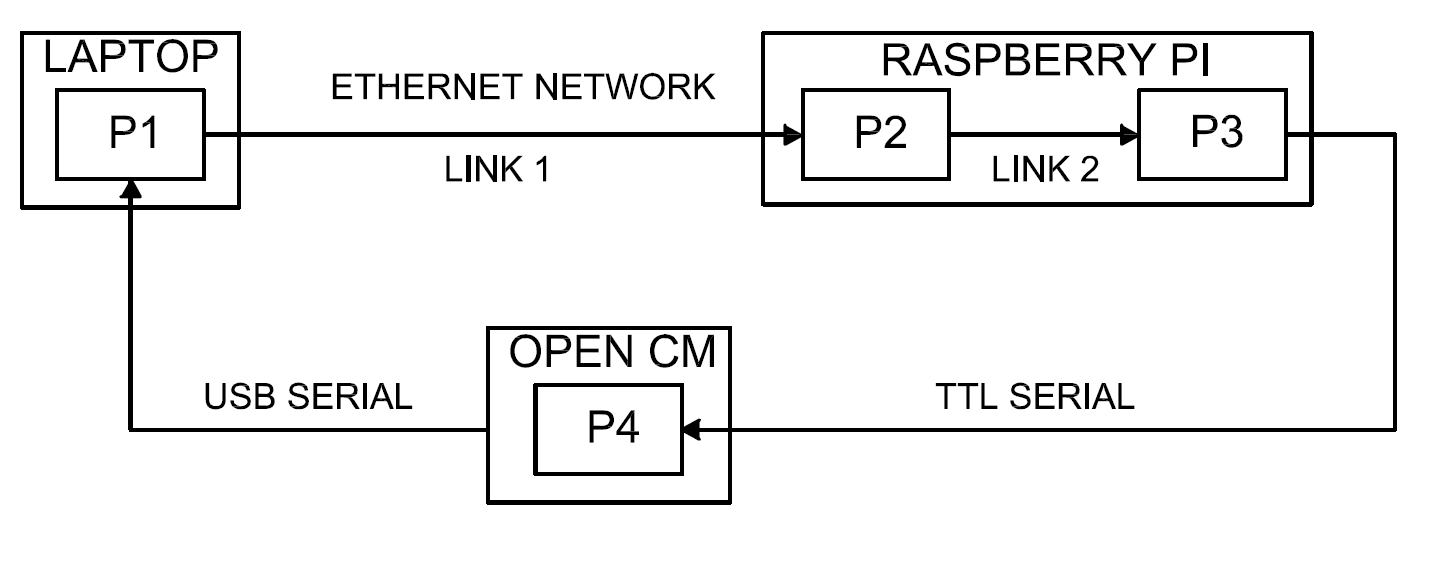
\includegraphics[width=1.0\columnwidth]{./images/testblock.png}
  \caption{Test Setup Block Diagram}
  \label{fig:test block diag}
\end{figure} 

Process P1 generates a random one byte message send sends the data over the network to process two. P2, P3, and P4 all have blocking read functions and immediately pass the message on to the next. This was done to simulate a more complex system while minimizing processing delays from the results. P1, P2, and P3 are written in Python while P4 was written in its native Arduino code. P1 utilizes the most accurate time function available to python. 10000 samples were processed for each test.

The objective was to simulate each IPCs ability to receive, process, and act on incoming sensor data. To accomplish this, the test was designed to send single byte messages at a high enough frequency to emulate sensor data without overloading each processor. As noted in the test results seen in prior research\cite{REALTIMEACH}, the initial communication of TCP can cause a spike in message latency. To eliminate this impact from our data we utilize a test message that must be successfully received prior to the start of data logging. 

The theoretical minimum latency for each communication link was evaluated to ensure the results obtained were a factor for the IPC method and not of processing delays and technology limitations. For the 100Mbps ethernet link, the theoretical transit time for a message would be 8 microseconds. Both the serial and USB communication links were set to 9600bps with a minimum transit time of 0.833 ms. This results in a total minimum latency of 1.675 ms for a single byte message. As the results will show, recorded latency ranged from 3 to 6 ms. All data being recorded well above the theoretical min concludes that the test yeilds viable results.
